%{{{ Image directe
\begin{frame}[t]
  \frametitle{Image directe}

  \begin{block}{Image directe}
    Soit $f: E\rightarrow F$ une application, et $\mathbf{A}$ une partie de $E$.
    On note l'\alert{\textbf{image directe}} de $A$ par $f$ l'ensemble:
    
    \begin{equation}
      f(A) = \left\{ f(x)\;|\; x\in E\right\}
    \end{equation}
  \end{block}
  \begin{columns}
    \begin{column}{0.5\textwidth}
      \begin{center}   
        \begin{tikzpicture}
   \node[ellipse, minimum width=1.5cm, minimum height=2.5cm, draw,
     thick, label=left:$E$] at(0,0)  {};
   \node[ellipse, minimum width=1.5cm, minimum height=2.5cm, draw,
     thick, label=right:$F$] at(3,0)  {};
   \node[point, fill=sexyRed!80] (A) at (0.2,0.5){};
   \node[point, fill=sexyRed!80] (B) at (0.1,0.0){};
   \node[point, fill=sexyRed!80] (C) at (-0.15,-0.4){};

   \node[point, fill=Apricot,xshift=3cm ] (fA) at (0.2,0.5){};
   \node[point, fill=Apricot,xshift=3cm] (fB) at (0.1,0.0){};
   \node[point, fill=Apricot,xshift=3cm] (fC) at (0.15,-0.6){};

   \path[->,>=stealth, thick] (A) edge[bend left=45] (fA);
   \path[->,>=stealth, thick] (B) edge[bend left=35] (fB);
   \path[->,>=stealth, thick] (C) edge[bend right=35] (fB);
   \node[draw=Apricot, thick, fit=(A)(B), rounded corners,label=left:$A$]{};
   \node[draw=sexyRed, thick, fit=(fA)(fB), rounded corners]{};
   \node at (3,1){\tiny$f(A)$};
 \end{tikzpicture}
 \end{center}
    \end{column}
    \begin{column}{0.5\textwidth}
      \begin{center}      
        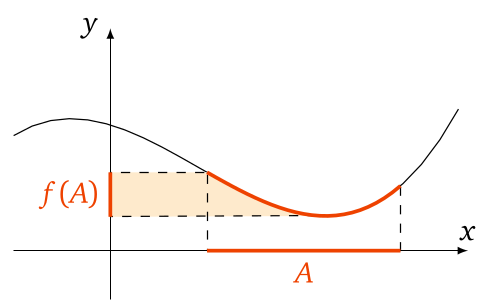
\includegraphics[width=4.5cm, height=3.5cm]{./image_directe.png}
\end{center}
    \end{column}
  \end{columns}
\end{frame}
%}}}
% Image réciproque {{{ %
\begin{frame}[t]
  \frametitle{Image Réciproque}

  \begin{block}{Image directe}
    Soit $B\subset F$ et $f:E\rightarrow F$ une application de $E$ dans $F$. On
    définit \textbf{\alert{l'image réciproque}} de $B$ par f: 
    
    \begin{equation}
      f^{-1}(B) = \left\{ x \in A\;|\; f(x)\in B\right\}
    \end{equation}
  \end{block}
  \begin{columns}
    \begin{column}{0.5\textwidth}
      \begin{center}   
        \begin{tikzpicture}
   \node[ellipse, minimum width=1.5cm, minimum height=2.5cm, draw,
     thick, label=left:$E$] at(0,0)  {};
   \node[ellipse, minimum width=1.5cm, minimum height=2.5cm, draw,
     thick, label=right:$F$] at(3,0)  {};
   \node[point, fill=sexyRed!80] (A) at (0.2,0.5){};
   \node[point, fill=sexyRed!80] (B) at (0.1,0.0){};
   \node[point, fill=sexyRed!80] (C) at (-0.15,-0.4){};

   \node[point, fill=Apricot,xshift=3cm ] (fA) at (0.2,0.5){};
   \node[point, fill=Apricot,xshift=3cm] (fB) at (0.1,0.0){};
   \node[point, fill=Apricot,xshift=3cm] (fC) at (0.15,-0.6){};

   \path[->,>=stealth, thick] (A) edge[bend left=45] (fA);
   \path[->,>=stealth, thick] (B) edge[bend left=35] (fB);
   \path[->,>=stealth, thick] (C) edge[bend right=35] (fB);
   \node[draw=Apricot, thick, fit=(fB)(fC), rounded corners,label=right:$B$]{};
   \node[draw=sexyRed, thick, fit=(B)(C), rounded corners]{};
   \node at (0,-0.8){\scriptsize$f^{-1}(B)$};
 \end{tikzpicture}
 \end{center}
    \end{column}
    \begin{column}{0.5\textwidth}
      \begin{center}      
        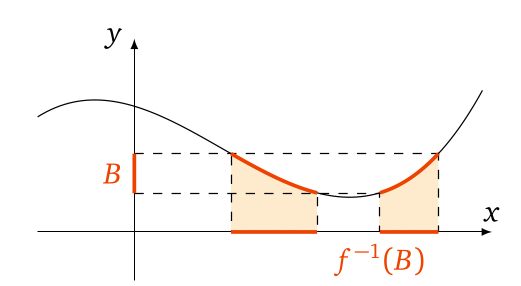
\includegraphics[width=4.5cm, height=3.5cm]{./image_reciproque.png}
\end{center}
    \end{column}
  \end{columns}
\end{frame}
% }}} Image réciproque %

% Antécédants {{{ %
\begin{frame}[t]
  \frametitle{Antécédents}
  
  \begin{block}{Antécédent}
    Soit une application $f:E\rightarrow F$ et $y\in F$. Un élément $\mathbf{x}$
    est un \textbf{\alert{antécédent}} de $y$ si on as 
    \begin{equation*}
      y = f(x)
    \end{equation*}
  \end{block}
  \begin{columns}
    \begin{column}{0.5\textwidth}
      \begin{center}   
        \begin{tikzpicture}
   \node[ellipse, minimum width=1.5cm, minimum height=2.5cm, draw,
     thick, label=left:$E$] at(0,0)  {};
   \node[ellipse, minimum width=1.5cm, minimum height=2.5cm, draw,
     thick, label=right:$F$] at(3,0)  {};
   \node[point] (A) at (0.2,0.5){};
   \node[point, fill=sexyRed!80,label=left:$x_1$] (B) at (0.1,0.0){};
   \node[point, fill=sexyRed!80,label=left:$x_2$] (C) at (-0.15,-0.4){};
   \node[point, fill=sexyRed!80,label=left:$x_3$] (D) at (-0,-0.7){};

   \node[point, fill=Apricot,xshift=3cm ] (fA) at (0.2,0.5){};
   \node[point, fill=Apricot,xshift=3cm, label=right:$y$] (fB) at (0.1,0.0){};
   \node[point, fill=Apricot,xshift=3cm] (fC) at (0.15,-0.6){};

   \path[->,>=stealth, thick] (A) edge[bend left=45] (fA);
   \path[->,>=stealth, thick] (B) edge[bend left=35] (fB);
   \path[->,>=stealth, thick] (C) edge[bend right=35] (fB);
   \path[->,>=stealth, thick] (D) edge[bend right=35] (fB);
 \end{tikzpicture}
 \end{center}
    \end{column}
    \begin{column}{0.5\textwidth}
      \begin{center}      
        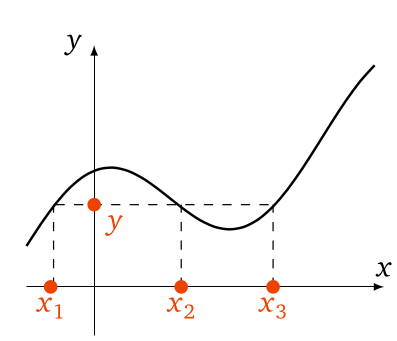
\includegraphics[width=4.5cm, height=3.5cm]{./antecedent.png}
\end{center}
    \end{column}
  \end{columns}
\end{frame}
% }}} Antécédants %
% Mini exercices {{{ %
\begin{frame}[<+->]
  \frametitle{Mini exercices}
  \small
  \begin{itemize}
    \item Soient $f$ et $g: E\rightarrow F$ deux applications. Donner la
      \textbf{négation}   de $f=g$.
    \item Représenter le graphe de la fonction $f:\N\rightarrow\R$ définie par
      $f(n)=\dfrac{4}{n+1}$
    \item Soient $f, g$ et $h: \R\rightarrow\R$ définies par:
      \begin{itemize}
        \item $f(x) = x^2$
        \item $g(x) = 2x + 1$
        \item $h(x) = x^3 - 1$
      \end{itemize}
      Donner l'expression des fonctions suivantes: $f\circ\left(h\circ h\right)$ et
      $\left(f\circ g\right)\circ h$
      \item Soit la fonction $f:\R\rightarrow\R$ définie par $f(x)=x^2$. Donner
        les ensembles suivants: $f([0,1[)$, $f(\R)$, $f(]-1,2[)$,
        $f^{-1}([1,2[)$, $f^{-1}(]-1,1[)$, $f^{-1}(3)$.
  \end{itemize}
\end{frame}
% }}} Mini exercices %
